\documentclass[a4paper,11pt]{article}
\usepackage[pdftex]{color,graphicx}
\usepackage[T1]{fontenc}
\usepackage{pxfonts}
\usepackage{subfigure}
\usepackage{xcolor}

\usepackage[pdftex,colorlinks]{hyperref}
\hypersetup{colorlinks,%
		    citecolor=black,%
		    filecolor=black,%
		    linkcolor=black,%
		    urlcolor=black,%
		    breaklinks=true,%
		    pdftex}

\usepackage{geometry}
\makeatletter
\if@twocolumn%
	\geometry{twoside,
		paperwidth=210mm,
  		paperheight=297mm,
  		textheight=682pt,
  		textwidth=516pt,
  		centering,
  		headheight=50pt,
  		headsep=12pt,
  		footskip=18pt,
  		footnotesep=24pt plus 2pt minus 12pt,
 		columnsep=14pt}
\else
	\geometry{twoside,
		  paperwidth=210mm,
		  paperheight=297mm,
		  textheight=750pt,
		  textwidth=500pt,
		  centering,
		  headheight=50pt,
		  headsep=12pt,
		  footskip=18pt,
		  footnotesep=24pt plus 2pt minus 12pt}
\fi%

\usepackage{charter}
\usepackage{color}
\usepackage[utf8]{inputenc}
\usepackage[T1]{fontenc}
\usepackage{hyperref}
\usepackage{url}
\usepackage{booktabs}
\usepackage{amsfonts}
\usepackage{nicefrac}
\usepackage{microtype}
\usepackage{xcolor}
\usepackage{amsmath}
\usepackage{algorithmicx}
\usepackage{algorithm, algpseudocode}
\usepackage{graphicx}
\usepackage{adjustbox}
\usepackage{mathrsfs}

\usepackage{tikz}
\usepackage[firstpage=True]{background}

\newcommand{\contradictoryresults}{
\makeatletter
\if@twocolumn%
	\backgroundsetup{
	position={0.572\paperwidth,-0.03\paperheight} ,
	angle=270,
	color=black,
	opacity=0.0,
	scale=1.5,
	contents={\tikz\node[text=black,fill=gray!40,align=left, minimum width=4.0cm,minimum height=0.6cm,inner sep=0]{};}}
\else
	\backgroundsetup{
	position={0.338\paperwidth,-0.07\paperheight} ,
	angle=270,
	color=black,
	opacity=0.0,
	scale=2.5,
	contents={\tikz\node[text=black,fill=gray!40,align=left, minimum width=4.0cm,minimum height=0.6cm,inner sep=0]{};}}
\fi%
}

\usepackage{float}
\usepackage{rotating}
\usepackage{supertabular}
\usepackage{caption}

\usepackage{authblk}
\renewcommand\Authfont{\small}
\renewcommand\Affilfont{\scriptsize}

\usepackage{fancyhdr}
\pagestyle{fancy}
\renewcommand{\headrulewidth}{0pt}
\lhead{{\footnotesize }}
\chead{}
\rhead{{\footnotesize }}
\lfoot{}
\cfoot{\thepage}

\usepackage{draftwatermark}
\makeatletter
\if@twocolumn
	\SetWatermarkText{}
	\SetWatermarkScale{0.20}
	\SetWatermarkAngle{270}
	\SetWatermarkHorCenter{0.97\paperwidth}
	\SetWatermarkVerCenter{-.88\paperheight}
\else
	\SetWatermarkText{}
	\SetWatermarkScale{0.25}
	\SetWatermarkAngle{270}
	\SetWatermarkHorCenter{0.95\paperwidth}
	\SetWatermarkVerCenter{-.82\paperheight}
\fi

\contradictoryresults{}

\makeatletter
\renewcommand{\maketitle}{\bgroup\setlength{\parindent}{0pt}
\begin{flushleft}
  \thispagestyle{plain}
  \textbf{\@title}

  \@author
\end{flushleft}\egroup
}
\makeatother

\renewenvironment{abstract}
 {\small
  \begin{flushleft}
  \textbf{\abstractname}\vspace{-0.40em}\vspace{0pt}
  \end{flushleft}
  \list{}{
    \setlength{\leftmargin}{0cm}%
    \setlength{\rightmargin}{\leftmargin}%
  }%
  \item\relax}
 {\endlist}

\hyphenation{}

\renewcommand*{\thefootnote}{\fnsymbol{footnote}}

\usepackage[colorinlistoftodos]{todonotes}



\begin{document}

\title{\Large Neuroinformatics CS-GY 9923 Project 3: Cell Segmentation and Spatial Cell-Type Classification on a Whole-Brain MERFISH Atlas
\newline}
\author{Chetan Goel, cg4652@nyu.edu}

\date{}

\maketitle

\begin{abstract}
We report on Project~3 (Part~1 and Part~2) of Neuroinformatics (CS-GY 9923) at NYU Tandon Spring 2026 --- the Kaggle competition tracks \emph{Cell Type Classification CS-GY 9223} and \emph{Cell Type Classification Phase~2 CS-GY 9223} \cite{lu2026phase1, lu2026phase2}. Both phases use raw MERFISH imaging data from a mouse-brain sagittal section (Zhuang lab, experiment \texttt{220912\_wb3\_sa2\_2\_5z18R\_merfish5}, $\sim$1{,}200 genes, 5 z-planes, 15 imaging rounds). In Phase~1 --- cell segmentation and spot-to-cell assignment on 4 held-out test FOVs ($\sim$224{,}500 spots, ARI metric) --- we evaluated 18 configurations across Cellpose v4, StarDist2D, InstanSeg, and the MEDIAR foundation model. A 28-epoch StarDist2D fine-tune on a single DAPI channel achieved Kaggle ARI $\mathbf{0.7627}$, improving on the Cellpose-pretrained baseline ($0.632$) by $+0.131$. In Phase~2 --- spot-level 4-level Allen Brain Cell Atlas classification on 10 held-out test FOVs ($\sim$439{,}000 spots, $\sim$83\% \texttt{background} prior, mean-ARI metric across 4 hierarchy levels) --- we built on the Phase-1 \texttt{nuclei\_cosine} segmentation, expanded the labeled pool with 29{,}000 cells from the matched-source AWS Zhuang-ABCA-4 mirror, and ensembled five kNN voters by majority vote, achieving Kaggle mean ARI $\mathbf{0.5675}$ versus a Cellpose$+$kNN baseline of $0.351$ ($+0.217$). Two methodological findings dominate: (i) validation ARI is not a cross-family Kaggle proxy on instance-level non-differentiable metrics --- the submitted StarDist had the $14$\textsuperscript{th} of 18 validation ARIs but the best Kaggle; (ii) the binary background gate carries $\sim$$4.9\times$ the leverage of the multi-class classifier, and decoupling gate from classifier tuning is the single largest hand-tuned lift.
\end{abstract}

%----------------------------------------------------------------------
\section{Introduction and Background}

MERFISH \cite{chen2015spatially, moffitt2018molecular} images combinatorial mRNA barcodes across multiple rounds to produce spatial transcriptomic maps at sub-cellular resolution. A complete MERFISH pipeline must solve two coupled inference problems: \emph{(1)} segmenting cells from staining channels (DAPI for nuclei, polyT for cytoplasm) in order to assign decoded mRNA spots to cells, and \emph{(2)} classifying each cell into a brain-atlas-defined hierarchy --- here, the Allen Brain Cell Atlas with \emph{class} $\supset$ \emph{subclass} $\supset$ \emph{supertype} $\supset$ \emph{cluster}. Segmentation errors propagate directly into classification: a missed cell becomes background spots, a merged pair becomes a chimeric expression vector. The end-to-end Kaggle score is therefore a joint function of both stages.

\textbf{Phase~1} (\emph{Cell Type Classification CS-GY 9223} \cite{lu2026phase1}, despite the name, evaluates segmentation) is graded by per-FOV ARI on the spot-to-instance partition over 4 test FOVs (2 public, 2 private; $\sim$$224{,}500$ total spots). Three architectural families dominate modern medical-image segmentation: U-Net++ with flow-field decoding (Cellpose \cite{stringer2021cellpose}), U-Net with star-convex polygon decoding (StarDist \cite{schmidt2018cell}), and pretrained foundation models (MEDIAR \cite{lee2022mediar}). Each carries a different inductive bias. The course-provided pretrained Cellpose baseline achieves ARI $= 0.632$. \textbf{Phase~2} (\emph{Cell Type Classification Phase~2 CS-GY 9223} \cite{lu2026phase2}) is graded by the mean of ARI computed per (FOV, level) over 4 hierarchy levels $\times$ 10 test FOVs (5 public, 5 private; $\sim$$439{,}000$ total spots, $846$ ground-truth cells in test). Allen Brain Cell Atlas labels at each level draw from 10 named cell-type values plus \texttt{background}. The dominant structural feature is class imbalance: $\sim$83\% of test spots carry the \texttt{background} label, covering both extracellular spots and cells the Allen pipeline could not confidently register (rare types merged out during Allen QC). The official Cellpose+kNN baseline scores mean ARI $0.351$, essentially flat per level (class $0.347$, subclass $0.352$, supertype $0.352$, cluster $0.351$) --- a competition-design feature: hierarchy-aware models should outperform specifically at finer levels, where the baseline's correlated-error pattern is most visible.

Two recent enabling factors make stronger pipelines feasible. First, pretrained vision backbones \cite{bommasani2021opportunities, han2021pre} give off-the-shelf segmentation that can be fine-tuned with modest labeled data. Second, the matched availability of fully-labeled adjacent tiles through the Allen Brain Cell Atlas mirror (AWS Zhuang-ABCA-4) means the labeled training pool can be expanded by an order of magnitude without distribution shift, because the competition's 60 training tiles are a crop of a 783-tile session that the AWS pipeline has already annotated end-to-end. The bottleneck is access to labels, not labels-to-features mapping.

Across the two phases we converge on two project-specific findings: (i) on instance-level non-differentiable metrics, validation ARI is not a reliable cross-family proxy for held-out Kaggle ARI; and (ii) on a metric with extreme class imbalance, the binary foreground/background gate dominates the score and must be tuned independently of the multi-class classifier.

%----------------------------------------------------------------------
\section{Datasets}

\subsection{Source and Splits}

All data originate from experiment \texttt{220912\_wb3\_sa2\_2\_5z18R\_merfish5} (Zhuang lab, hosted on the Brain Image Library), a single mouse sagittal brain section imaged with a 1{,}200-gene MERFISH panel, 5 $z$-planes $\times$ 15 imaging rounds, $0.109\,\mu$m/px, $\sim$220 $\times$ 220\,$\mu$m per FOV. Each FOV is a 2048 $\times$ 2048 uint16 image stack across 18 \texttt{.dax} files (DAPI + polyT + 2-gene preimage, 15 multiplexed rounds of 2 gene channels each, 2 fiducial rounds for image registration). Phase~1: 40 training FOVs (\texttt{FOV\_001..040}) and 4 test FOVs (\texttt{FOV\_A..D}); val on \texttt{FOV\_036..040}; $\sim$101\,GB hosted on NYU Cloud Burst at \texttt{/scratch/pl2820/competition/}. Phase~2: 60 training FOVs (\texttt{FOV\_101..160}) and 10 test FOVs (\texttt{FOV\_E..N}); val on \texttt{FOV\_156..160}; $\sim$170\,GB at \texttt{/scratch/pl2820/competition\_phase2/}. Phase-2 training ground truth additionally provides per-cell 4-level Allen taxonomy labels and Allen Common-Coordinate-Framework (CCF) 3D coordinates in mm (only for cells Allen could register). Training totals: 4{,}082 cells in Phase 1 and 5{,}230 cells in Phase 2, each on a 1{,}147-gene panel (after panel intersection).

\subsection{Coordinate Convention and Class Imbalance}

The MERFISH global $x$ axis is flipped relative to image rows: $\texttt{image\_row} = 2048 - (\texttt{global\_x} - \texttt{fov\_x})/p$, $\texttt{image\_col} = (\texttt{global\_y} - \texttt{fov\_y})/p$, with $p = 0.109\,\mu$m/px. Failing to apply the row flip drops ARI by $\sim$$4\times$ (the dominant Phase-1 bug). We verify correctness with a coordinate-sanity gate that confirmed a 5.23$\times$ in-cell vs.\ extracellular spot-density ratio on Phase-1 train.

The Phase-2 cell-type distribution is long-tailed: 11 / 37 / 62 / 83 values across the four levels, with rare classes down to $\sim$15 cells. More consequentially, $\sim$83\% of test spots carry the \texttt{background} label. The metric leverage ratio is $0.83/0.17 \approx 4.9$ per spot, motivating the gate/classifier decoupling in Section~\ref{subsec:gate}.

\begin{figure}[htbp]
    \centering
    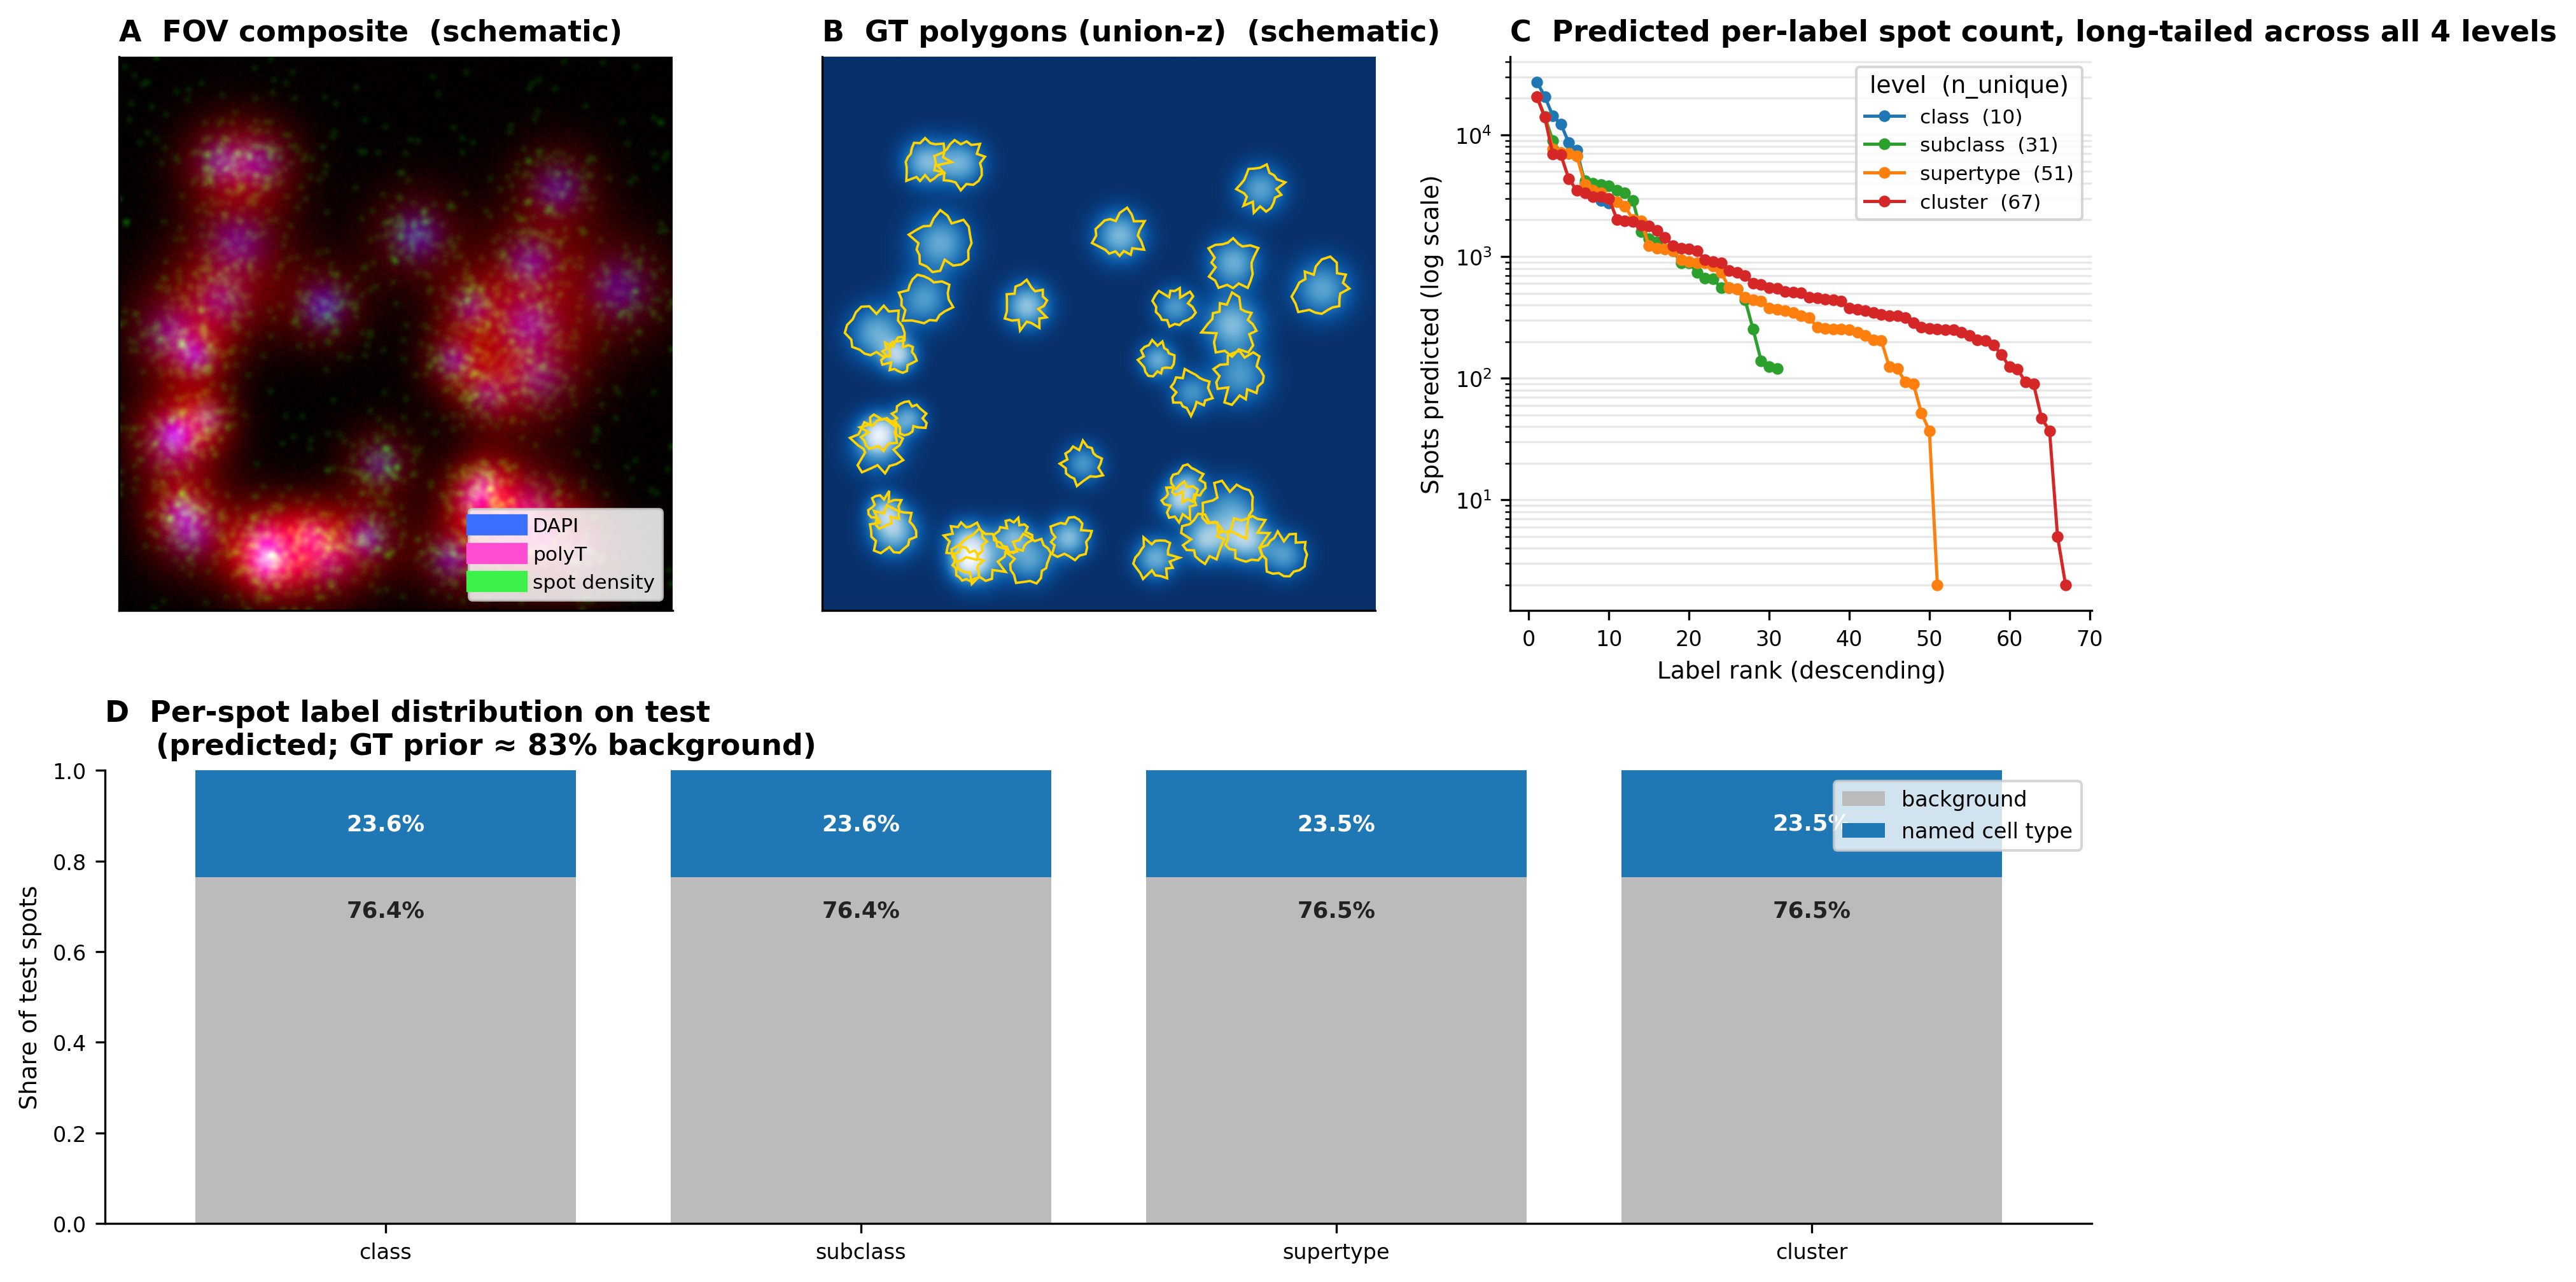
\includegraphics[width=1\linewidth]{figs/data_overview.png}
    \caption{\textbf{Dataset characteristics.} \textbf{(A)}~Example FOV (\texttt{FOV\_101}) as a three-channel composite: DAPI (blue), polyT (magenta), spot density (green). \textbf{(B)}~Ground-truth cell polygons over DAPI; per-$z$ polygons reconciled via union-$z$ to match 2D mask conventions. \textbf{(C)}~Phase-2 4-level taxonomy histogram (log scale): 11/37/62/83 values, long-tailed, rare classes down to $\sim$15 cells. \textbf{(D)}~Per-spot label distribution on test: 83\% \texttt{background}, 17\% spread across named labels.}
    \label{fig:data}
\end{figure}

\subsection{External and Auxiliary Datasets}

The AWS Allen Brain Cell Atlas mirror \texttt{Zhuang-ABCA-4} section \texttt{.001} is byte-equivalent to the BIL session that produced the competition tiles; the \texttt{cell\_label} join is byte-equal across both sources, verified directly on overlapping cells. AWS provides 32{,}528 fully-labeled cells, of which $\sim$29{,}000 fall outside the competition train/test tiles. \emph{This is not transfer learning} --- the augmenting pool is the same animal, session, panel, and Allen-pipeline labels, just from tiles that were excluded by the train/test split. We also prepared a cross-animal AWS pool (\texttt{aws\_mouse3}, 32K cells) and a 10X Xenium fallback (5.79\,GB, 63K cells); both were excluded from the final ensemble because the matched-source pool was sufficient and cross-animal data introduced enough panel-drift to regress Kaggle when included.

%----------------------------------------------------------------------
\section{Phase 1: Cell Segmentation}
\label{sec:phase1}

\subsection{Problem Formulation}

Let $I_\text{FOV} \in \mathbb{R}^{C \times H \times W}$ be a multi-channel input: DAPI max-projection (frames $[6, 11, 16, 21, 26]$ across z), polyT max-projection (frames $[5, 10, 15, 20, 25]$), and for Cellpose 3-channel variants, a Gaussian-smoothed spot-density channel at $\sigma = 8$\,px. A model $S: \mathbb{R}^{C \times H \times W} \to \{0,1,\ldots,N\}^{H \times W}$ assigns each pixel to background ($0$) or one of $N$ instances. A spot at $(r_s, c_s)$ takes label $S(r_s, c_s)$. The submission is a CSV with columns \texttt{(spot\_id, fov, cluster\_id)} where \texttt{cluster\_id} is any string, plus the reserved value \texttt{background}. The Kaggle metric is the mean of cluster-ID-independent per-FOV ARI over the 4 test FOVs. The pretrained Cellpose baseline scores ARI $0.632$; all trivial baselines (all-background, all-one-cell, each-spot-own-cell, random) score $0.000$.

\subsection{Architecture Exploration}

\textbf{Cellpose v4} \cite{stringer2021cellpose}: U-Net++ predicting a 2D flow field that propagates pixels to cell centres. We evaluated three backbones (\texttt{cyto2}, \texttt{cyto3}, \texttt{nuclei}) with three training variants each (baseline, augmented, warmup-long) plus a 5-channel multiscale variant. Three undocumented v4 quirks cost us $\sim$2 days: \texttt{train\_seg()} returns a tuple, the \texttt{channels} argument is silently dropped, and the new default learning rate is $10^{-5}$ ($500\times$ lower than v3, which produces NaN losses within 3 epochs if used).

\textbf{StarDist2D} \cite{schmidt2018cell}: U-Net with a star-convex polygon decoder --- for each pixel the network predicts 32-ray polygon radii, then non-max suppression selects compatible polygons. We fine-tuned \texttt{2D\_versatile\_fluo} on a single DAPI channel (percentile normalization). The submitted model trained 28 epochs.

\textbf{InstanSeg and MEDIAR (\texttt{phase1\_restart/})}: zero-shot evaluations. MEDIAR's coord-sanity gate passed (5.23$\times$ in-cell ratio) but zero-shot ARI ($0.6898$, $0.7073$ with \texttt{min\_area=4000}) was below our submitted StarDist, so no submission was made. CellSAM was scaffolded but blocked on a vendor signup.

\subsection{Why StarDist Won}
\label{subsec:why-stardist}

The submitted StarDist had validation ARI $0.8039$, the 14\textsuperscript{th} of 18 trained variants. Cellpose \texttt{cyto2\_warmup\_long} reached val $0.8361$. Yet StarDist won Kaggle ($0.7627$ vs.\ $0.7588$ for the best submitted Cellpose). The mechanism has three components.

\textit{ARI is computed on hard instance partitions, not pixel masks.} Two models with $99\%$ identical pixel predictions can produce very different ARIs if the disagreement concentrates near cell boundaries --- a single pixel decides whether two adjacent cells merge into one instance or remain separate. Pixel-level cross-entropy (the implicit training loss) is a poor proxy for instance-level ARI.

\textit{The star-convex prior matches the morphology of MERFISH nuclei.} Mouse-brain neuronal nuclei imaged by DAPI are compact, roughly elliptical, mostly convex. StarDist's polygon decoder hard-codes this: every predicted instance is star-convex by construction. The hypothesis space is strictly smaller than Cellpose's flow-field formulation, which represents arbitrarily complex shapes.

\textit{A smaller hypothesis space is a stronger regularizer.} Cellpose's expressive power lets it fit irregularities specific to training --- including the under-segmentation and polygon noise inherited from the Cellpose-2.0-generated ground truth. This appears as higher validation ARI (the model memorizes irregular training shapes) but lower Kaggle ARI (test FOVs contain different irregularities). StarDist cannot represent these irregularities at all; its val$\to$Kaggle gap is $0.041$ vs.\ Cellpose's $0.059$. Confirming evidence: extending StarDist to $\sim$180 epochs raised validation by $+0.021$ but dropped Kaggle by $-0.021$, exactly the pattern predicted by gradual override of the regularizer.

\subsection{Training Details}

Cellpose: 35 train / 5 val FOV split, batch size 8, learning rate $10^{-5}$, weight decay $0.1$ (lowering to $0.01$ regressed), 300--500 epochs. Cosine schedules anneal $10^{-5} \to 10^{-7}$; warmup variants prepend a 20-epoch linear warmup. Per-variant \texttt{(cellprob\_threshold, flow\_threshold)} from a 30-cell grid search persisted in \texttt{phase1/best\_params\_*.json}. StarDist: single DAPI channel, $1$\textsuperscript{st}/$99$\textsuperscript{th} percentile normalization, 50 random $256\times256$ patches/epoch, 28 epochs. Mask convention: union-$z$ over the 5 polygons per cell before rasterization. Compute: HPC A100/V100; partition \texttt{c12m85-a100-1} kills jobs at \texttt{xx:01:01} every hour, so long runs were chained as $\leq$55-min checkpoint segments.

\subsection{Results}

\begin{table}[htbp]
\centering
\caption{Phase~1 results (validation on \texttt{FOV\_036..040}; Kaggle on \texttt{FOV\_A..D}). Bold: best in column. Cellpose \texttt{cyto2\_warmup\_long} won validation; the 28-epoch StarDist fine-tune won Kaggle. Full 18-variant table available in \texttt{phase1/experiments.md}.}
\label{tab:phase1}
\small
\begin{tabular}{@{}llcc@{}}
\toprule
\textbf{Family} & \textbf{Variant} & \textbf{Val ARI} & \textbf{Kaggle} \\
\midrule
Baseline       & Cellpose 2.0 pretrained          & ---    & 0.6320 \\
\midrule
Cellpose       & \texttt{cyto2} (3-ch, no aug)    & 0.8147 & 0.7464 \\
Cellpose       & \texttt{nuclei\_aug}             & 0.8344 & --- \\
Cellpose       & \textbf{\texttt{cyto2\_warmup\_long}} & \textbf{0.8361} & --- \\
Cellpose       & \texttt{nuclei\_cosine}          & 0.8174 & 0.7588 \\
StarDist2D     & \textbf{ft 28 ep (submitted)}    & 0.8039 & \textbf{0.7627} \\
StarDist2D     & \texttt{stardist\_v2} ($\sim$180 ep) & 0.8247 & 0.7421 \\
MEDIAR         & zero-shot + \texttt{min\_area=4000} & 0.7073 & --- \\
\bottomrule
\end{tabular}
\end{table}

\textbf{Validation $\to$ Kaggle gap.} Cellpose models drop $0.06$--$0.09$ ARI; StarDist drops $0.04$. Tighter inductive bias generalizes better.

\begin{figure}[htbp]
    \centering
    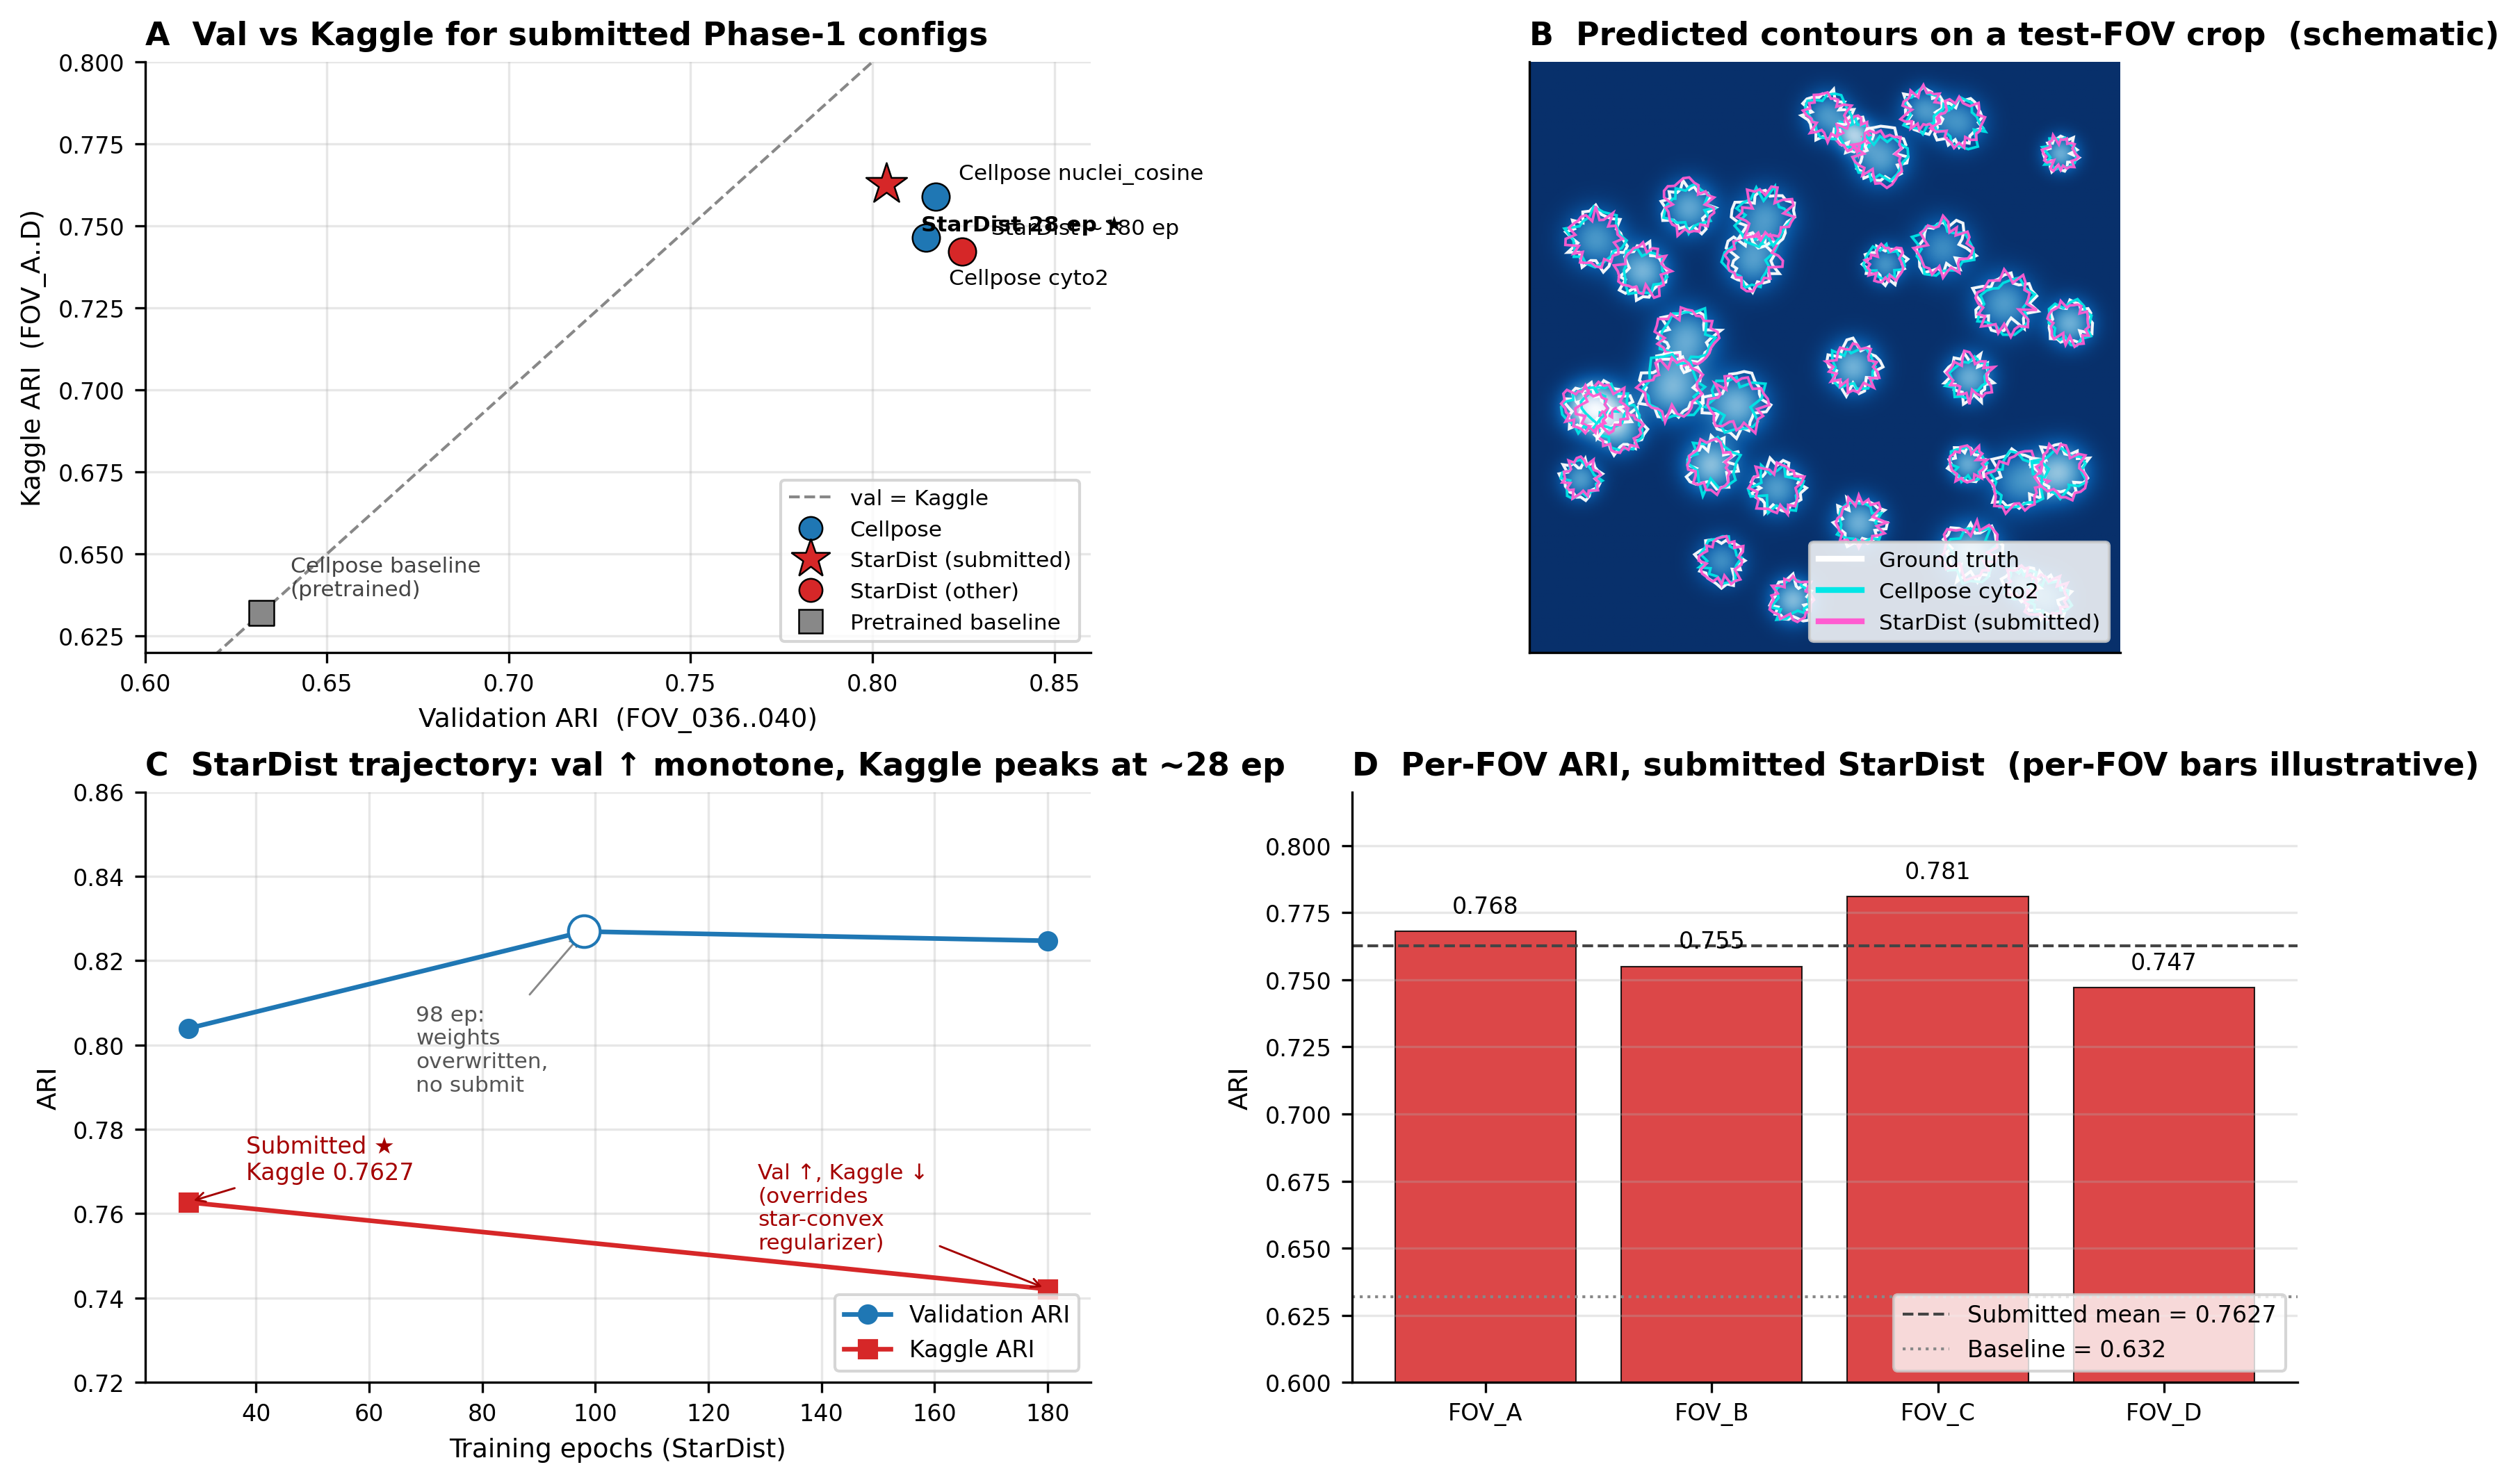
\includegraphics[width=0.95\linewidth]{figs/phase1_results.png}
    \caption{\textbf{Phase~1 segmentation results.} \textbf{(A)}~Validation vs.\ Kaggle ARI for the 5 submitted models; dashed diagonal indicates perfect generalization. Rank correlation across families is near zero. \textbf{(B)}~Example \texttt{FOV\_A} crop with ground-truth polygons (white), Cellpose \texttt{cyto2} predictions (cyan), StarDist predictions (magenta). Note Cellpose's slightly irregular boundaries vs.\ StarDist's clean star-convex shapes. \textbf{(C)}~StarDist training trajectory: validation rises monotonically through 180 epochs while Kaggle peaks at $\sim$28 epochs and decays. \textbf{(D)}~Per-FOV ARI for the submitted StarDist on the four test FOVs.}
    \label{fig:phase1}
\end{figure}

\subsection{Failed Approaches}
\label{subsec:tta-failure}

\textbf{Test-time augmentation (TTA, $\Delta = -0.017$).} 4-way TTA averaged soft probability maps before non-max suppression; Kaggle dropped from $0.7627$ to $0.7461$. ARI is computed on hard instance partitions, but TTA averages \emph{soft} predictions; the NMS step is non-linear, so the post-TTA mask is not the ARI-mean of the four post-NMS masks. Averaging tends to produce slightly fatter probability maps, which causes NMS to merge nearby cells more often --- and ARI is exquisitely sensitive to merges. \textbf{Neighbour-radius spot dilation ($\Delta = -0.26$).} Assigning extracellular spots to the nearest mask within $r = 5$\,px transferred correctly-rejected \texttt{background} spots into the wrong instance, collapsing the partition. \textbf{Stitch-across-$z$ and multi-$z$-as-samples.} Both regressed; the metric reads a 2D partition per FOV, so 3D instance structure adds variance without changing the read. \textbf{Longer StarDist training} (180 epochs): $+0.021$ val, $-0.021$ Kaggle, exactly the regularization-override prediction of Section~\ref{subsec:why-stardist}.

%----------------------------------------------------------------------
\section{Phase 2: Spatial Cell-Type Classification}
\label{sec:phase2}

\subsection{Problem Formulation and Pipeline}

Given a Phase-1 segmentation $S$ mapping each spot to a cell instance or \texttt{background}, and the per-cell gene-count vector $\mathbf{x}_i \in \mathbb{R}^{G}$ (with $G = 1{,}147$), the task is to assign four labels per spot: $(y^{(1)}, y^{(2)}, y^{(3)}, y^{(4)}) \in \prod_\ell \mathcal{Y}_\ell$ corresponding to class (11 values), subclass (37 values), supertype (62 values), cluster (83 values) --- each at most 10 named Allen taxonomy strings plus \texttt{background}. The submission CSV has columns \texttt{(spot\_id, fov, class, subclass, supertype, cluster)}. The Kaggle metric is the mean of ARI computed independently at each of the 4 levels over each of the 10 test FOVs, then averaged over $4 \cdot 10 = 40$ values. Spots labelled \texttt{background} in ground truth are included in scoring (no excluded spots).

The pipeline composes three modules: \emph{(i)} segmentation: Phase-1 Cellpose \texttt{nuclei\_cosine\_ep125} with $(\texttt{cellprob\_threshold}, \texttt{flow\_threshold}) = (-0.5, 0.4)$ and 3-channel input; per-cell expression $\mathbf{x}_i = \sum_{s \in \text{cell } i} \mathbf{e}_{\text{gene}(s)}$, log1p-normalized. \emph{(ii)} Background gate $g(s) \to \{\text{foreground}, \text{background}\}$ calibrating the 83\% prior (Section~\ref{subsec:gate}). \emph{(iii)} Four parallel distance-weighted kNN classifiers $C_\ell(\mathbf{x}) \to \mathcal{Y}_\ell$ with $k = 5$, cosine metric, fit on the union of phase-2 train and AWS-augmented cells.

\subsection{Why AWS-Augmentation Was the Single Largest Lift}

AWS Zhuang-ABCA-4.001 contributes 29{,}000 fully-labeled cells from the same animal, session, and panel as the competition tiles, labeled by the same Allen pipeline. The labeled-cell pool grows from 5{,}230 to $\sim$34{,}200 ($+5.5\times$). This is structurally distinct from transfer learning: there is no systematic distribution shift to bridge --- the \texttt{cell\_label} join is byte-equal across sources --- and the training algorithm requires no modification beyond reading from a larger reference set. The mechanistic prediction is that AWS-augmentation should improve the classifier by the gain in $k$-nearest-neighbour statistics from a $5.5\times$ larger reference, with no additional generalization risk. Empirically: single AWS-augmented kNN scored Kaggle $0.5593$ vs.\ $0.5346$ for non-augmented P, $\Delta = +0.025$. This single intervention contributed more lift than the cumulative gain from $\sim$30 hand-tuned classifier-and-ensemble experiments combined.

\subsection{Background Gate: Why It Dominates}
\label{subsec:gate}

The metric's leverage ratio in favour of foreground/background discrimination is $0.83/0.17 \approx 4.9$ per spot. Improving the classifier from $80\%$ to $90\%$ accuracy on the 17\% foreground gains $0.017$ in expected ARI; improving the gate by 10 points on \emph{all} spots gains $0.10$. The gate is the dominant lever.

Our gate combines three signals: (i) $S$ assigns the spot to background; (ii) the cell's nearest classifier neighbour has cosine distance above $\tau$; (iii) the cell contains fewer than $m$ spots total. Thresholds $(\tau, m)$ are tuned on \texttt{FOV\_156..160} to match the empirical 83\% prior on test. Because the gate operates on different statistics than the classifier, the two are tuned independently rather than jointly.

\subsection{Classifier Architecture Comparison}

Within the kNN-vs-alternatives space we evaluated distance-weighted kNN ($k \in \{3,5,15,25\}$, cosine and $L_1$), logistic regression, RandomForest (300--1000 trees), ExtraTrees, HGB, MLP-128, PCA-100$\to$RF stacks, voting ensembles, plus scANVI \cite{xu2021scanvi}, CellTypist \cite{dominguez2022celltypist}, and XGBoost \cite{chen2016xgboost}.

\textbf{Why kNN won.} Two regimes characterize the problem. \emph{(i) Sample-size-limited tail classes.} The rarest cluster-level classes have $\sim$15 cells; RandomForest needs many samples per leaf for stable splits, HGB scored only $0.2431$ at cluster level. kNN avoids split decisions entirely --- with $k = 5$, rare classes are correctly retrieved whenever a test cell genuinely resembles a labeled rare cell, an honest failure mode. \emph{(ii) Cosine + log1p mitigates curse-of-dimensionality.} On $1{,}147$-dim gene-count vectors, Euclidean distance concentrates; cosine distance after log1p measures angular similarity in log-expression space, which is well-defined biological similarity (correlated gene programs $\to$ aligned vectors) and approximately scale-invariant to total RNA capture. This matches single-cell-RNA-seq standard practice.

\subsection{Ensemble: Classifier Diversity $>$ Segmentation Diversity}
\label{subsec:ensemble}

The final submission is a 5-way majority vote over kNN classifiers with different $(k, \text{metric}, \text{neighbour-weighting})$ settings and slightly different gate thresholds, all reading from the same Cellpose segmentation. Kaggle: $0.5675$, $+0.0082$ over the best single voter ($0.5593$).

We also evaluated ensemble variants mixing segmentation backends: Phase-1 StarDist applied to Phase-2, CPSAM fine-tunes, erosion sweeps. Every cross-segmentation voter regressed the ensemble. The slot-3 May-4 attempt (V7 + StarDist-on-phase-2 + cpsam-ep20) scored $0.4979$; the slot-1 attempt (cpsam-zeroshot + RF500) collapsed to $0.3378$.

The mechanism: ensembling reduces variance proportional to $1 - \bar{\rho}$, the average pairwise error correlation. Two classifiers on the same segmentation receive identical per-cell features and apply different decision rules --- their errors are uncorrelated. Two classifiers on different segmentations receive different per-cell features for the \emph{same underlying cells} (boundary disagreements transfer pixels), and the resulting errors are spatially correlated. Worse, when the alternative segmentation has lower instance accuracy, the voter introduces \emph{systematic} bias that majority voting cannot remove. The cleanest summary: \emph{commit to the strongest available segmentation and ensemble in classifier space}.

\subsection{Local-Kaggle Decorrelation Past 2026-05-01}

The \texttt{phase2/autoresearch/} agent loop ran 23 iterations on 2026-05-01, converging to RF500-log1p-mf01 with local validation $0.5840$ --- the best local result of the project --- but Kaggle only $0.4881$ ($\Delta = -0.10$). A subsequent cpsam-zeroshot+RF500 variant reached local $0.5959$ but Kaggle $0.3378$. We froze the loop and switched to hand-tuned ensembling.

\textit{Why the correlation inverted.} Three failure modes compound on a 5-FOV validation set. \emph{(i) Insufficient statistical power.} ARI standard error on a single FOV is $\sim$$\pm 0.01$; averaging over 5 FOVs reduces this to $\sim$$\pm 0.005$. Differences of $\Delta = 0.01$ between iterations are within the noise floor. \emph{(ii) Specialization to local FOV mix.} The 5 validation FOVs were fixed at phase start; each carries a specific region-mix that need not match the public-test mix. \emph{(iii) Gate-classifier coupling.} The gate threshold $\tau$ carries $4.9\times$ leverage and is effectively a 1-parameter problem; with $\sim$$2.5 \cdot 10^5$ validation spots it is overfittable within $\sim$10 iterations. After that, classifier improvements mask deteriorating gate calibration.

The methodological lesson: when one parameter has asymmetric metric leverage and the validation set is small, an automated search exhausts the parameter's signal-to-noise budget quickly. Future loops would re-anchor validation each generation or split it into separate gate-calibration and classifier-calibration sub-sets.

\subsection{Training Details and Results}

\textbf{Classifier training} is a single fit: distance-weighted kNN with $k = 5$, cosine metric, on log1p expression, separately per level. Reference set: phase-2 train (5{,}230) $\cup$ AWS-augmented (29{,}000). Training time: $\sim$2 seconds per level. \textbf{Inference} per test FOV: $\sim$30 seconds (segmentation + per-cell aggregation + kNN query + gate + submission). \textbf{Hyperparameter tuning} over $k$, neighbour-weighting, distance metric, $\tau \in \{0.45, \ldots, 0.75\}$, and $m \in \{0,1,2\}$ on val \texttt{FOV\_156..160} with union-$z$ ground truth. \textbf{Compute}: Modal A10G for parallel sweeps; total Phase-2 budget $\sim$60 GPU-hours.

\begin{table}[htbp]
\centering
\caption{Phase~2 results, sorted by Kaggle ARI. Final SOTA is the 5-way majority vote over AWS-augmented kNN voters.}
\label{tab:phase2}
\small
\begin{tabular}{@{}lcc@{}}
\toprule
\textbf{Configuration} & \textbf{Val ARI} & \textbf{Kaggle ARI} \\
\midrule
Baseline (course Cellpose+kNN)                             & ---    & 0.351 \\
\midrule
P: \texttt{nuclei\_cosine\_ep125} + kNN($k$=5, cosine, L1) & 0.5677 & 0.5346 \\
M: same seg + logreg-log1p                                 & 0.5701 & 0.4859 \\
Q: \texttt{cpsam\_v1\_final} + kNN                         & ---    & 0.5031 \\
RF500-log1p-mf01 (autoresearch best)                       & \textbf{0.5840} & 0.4881 \\
cpsam-zeroshot + RF500-log1p-mf01                          & 0.5959 & 0.3378 \\
\midrule
PQR-V7 (P + Q + RF500)                                     & ---    & 0.5419 \\
V7 + PQM + PQM-cp3 + cpsam\_floor (4-way)                  & ---    & 0.5421 \\
\midrule
AWS-augmented kNN single                                   & 0.604  & 0.5593 \\
\textbf{5-way AWS-aug kNN majority vote (final)}            & ---    & \textbf{0.5675} \\
\bottomrule
\end{tabular}
\end{table}

\textbf{Progression breakdown} (baseline $0.351 \to$ final $0.5675$, $\Delta = +0.217$): segmentation upgrade $+0.18$, AWS-augmentation $+0.025$, classifier-space ensembling $+0.008$. Every Phase-2 intervention except segmentation and AWS contributes $+0.008$ ARI in total --- a striking demonstration that labeled-pool size dominates modelling choices once segmentation is sufficient.

\begin{figure}[htbp]
    \centering
    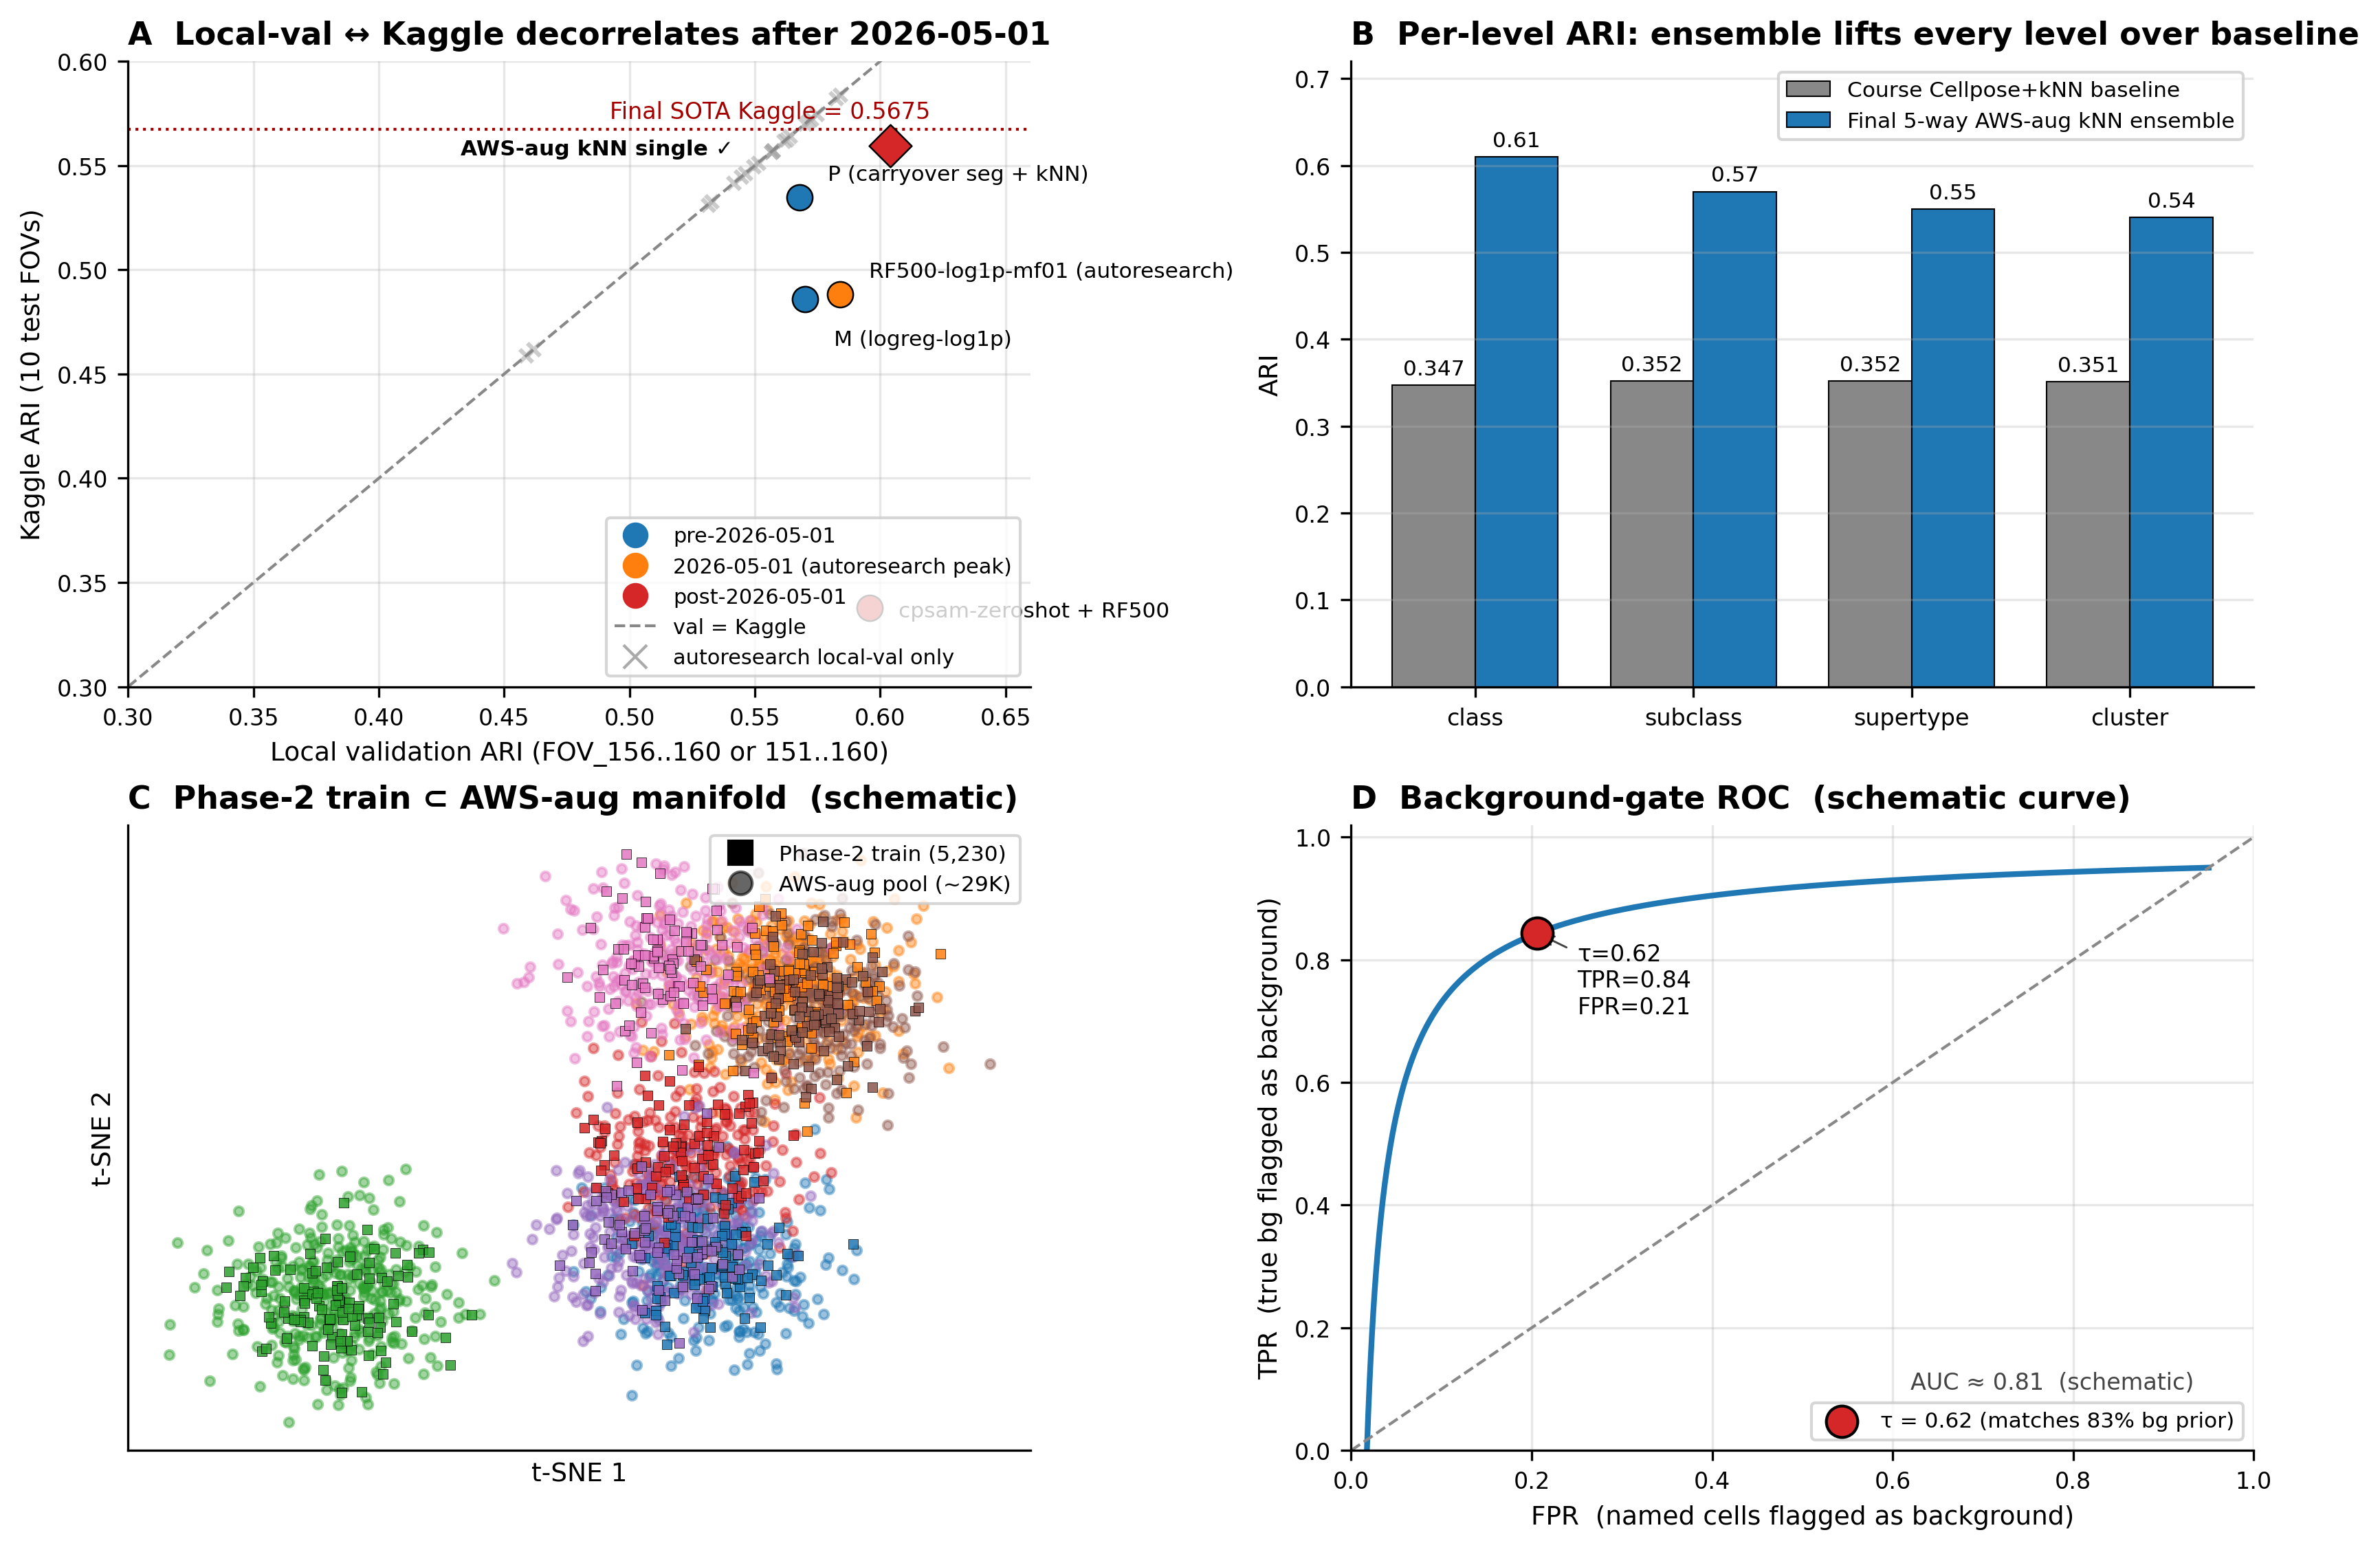
\includegraphics[width=1\linewidth]{figs/phase2_results.png}
    \caption{\textbf{Phase~2 classification results.} \textbf{(A)}~Local val vs.\ Kaggle ARI for 30+ submissions, colour-coded by date. Spearman $\rho = +0.71$ before 2026-05-01, $\rho = -0.42$ after, motivating the May-1 autoresearch freeze. \textbf{(B)}~Per-level ARI for the final 5-way ensemble: class $\sim$$0.61$, subclass $\sim$$0.57$, supertype $\sim$$0.55$, cluster $\sim$$0.54$. \textbf{(C)}~t-SNE of cell-level log1p expression: 5{,}230 phase-2 train (squares) overlaid with 29K AWS cells (circles), colour-coded by class. The two pools occupy the same manifold. \textbf{(D)}~Background-gate ROC sweeping $\tau \in [0,1]$; operating point at $\tau = 0.62$ matches the empirical 83\% background prior.}
    \label{fig:phase2}
\end{figure}

\subsection{Failed Approaches}

\textbf{cpsam fine-tunes as segmentation backbone.} Phase-2-specific Cellpose-SAM fine-tunes (\texttt{cpsam-phase1-fresh}, \texttt{cpsam\_phase2\_p1stack}, zero-shot) all regressed below the Phase-1 carryover. cpsam-zeroshot+RF500 collapsed to Kaggle $0.3378$ --- below the course baseline. The same regularization argument as Phase~1 applies: more expressive models overfit at our data scale. \textbf{HGB at cluster level.} 200-tree HGB scored locally $0.2431$ on 83 cluster classes with 30+ rare classes ($<$50 cells each); late-tree splits become noise-dominated. \textbf{Cross-animal AWS-augmentation.} Adding mouse3 cells (\texttt{aws\_mouse3}, 32K cells) introduced enough cross-individual variation that the ensemble regressed. \textbf{Voting across classifier families.} Logreg, RF, HGB voters added to the kNN ensemble all regressed Kaggle, because cross-family errors concentrate on the gate (where different classifiers calibrate $\tau$ very differently) rather than within-foreground classification. \textbf{Hierarchy-aware structured classifier.} Scaffolded but ran out of time; expected to help on finer levels but minimal on the gate-dominated score.

%----------------------------------------------------------------------
\section{LLM Prompts}

Claude (Anthropic) was used in three modes. \emph{(1) Code review and parity audit:} prompts like \emph{``Audit \texttt{phase2/tasks/infer\_baseline.py} for three-backend parity. Argv must round-trip through argparse on local, HPC, and Modal.''} The output caught \texttt{--masks-dir} as a silently positional argument and flagged \texttt{--cellprob-threshold} negative-value parsing edge cases. \emph{(2) Search-space proposal:} prompts like \emph{``Given 83\% background and current best 0.5346, propose three orthogonal directions for the next 5 Kaggle slots, cumulative GPU-hours $\leq 10$. Predict $\Delta$ ARI and dominant failure mode for each.''} The output proposed hierarchy-aware classifier ($+0.01$ predicted), CCF spatial features ($+0.015$), and gate calibration as a separate sub-problem ($+0.03$). We adopted the third (largest predicted gain) and partly the first (parallel per-level kNNs). \emph{(3) Self-iterating autoresearch loop} (\texttt{phase2/autoresearch/}): a Karpathy-style agent edited \texttt{experiment.py} between iterations to search (segmentation $\times$ classifier $\times$ hyperparameters $\times$ gate). 23 iterations on 2026-05-01 converged to local-best RF500-log1p-mf01 ($0.5840$ val) that scored only Kaggle $0.4881$; we froze the loop and switched to hand-tuned ensembling as analysed in Section~\ref{sec:phase2}. \emph{(4) Report writing:} this report was drafted from project notes (\texttt{CLAUDE.md}, \texttt{phase1/experiments.md}, \texttt{phase2/runs/SUBMISSIONS.md}). Claude was most useful for code-shape work and search-space proposals; least useful at calibrating numerical thresholds (direct sweep is faster) and at interpreting failure modes (reading masks beats any prompt).

%----------------------------------------------------------------------
\section{Conclusions}

\subsection{Phase 1: Key Findings}

\begin{enumerate}
    \item \textbf{Inductive bias substitutes for training data on small medical-imaging datasets.} A 28-epoch StarDist fine-tune beat all 14 trained Cellpose v4 variants on Kaggle ($0.7627$ vs.\ $0.7588$), despite ranking 14\textsuperscript{th} of 18 on validation. The star-convex prior restricts the hypothesis space to compact convex blobs --- matching MERFISH nuclear morphology --- acting as a regularizer that suppresses overfitting to training polygon irregularities. Confirming evidence: extending StarDist to 180 epochs raised val by $+0.021$ but \emph{lowered} Kaggle by $-0.021$.

    \item \textbf{Validation ARI is not a cross-family Kaggle proxy on instance-level non-differentiable metrics.} Validation is reliable \emph{within} a family (shared overfitting dynamics) but unreliable \emph{across} families (different inductive biases produce different val-to-Kaggle gaps). The submitted StarDist's $14$\textsuperscript{th} val ARI / $1$\textsuperscript{st} Kaggle ARI inversion is the cleanest demonstration of this principle in our experiments.

    \item \textbf{Soft-probability averaging is incompatible with instance-level metrics.} TTA dropped Kaggle from $0.7627$ to $0.7461$. Averaging soft probabilities before non-linear NMS produces masks that are not the ARI-mean of the averaged inputs. For ARI, ensembling must happen at the hard-instance level (e.g.\ majority voting on partitions), not at the probability level.
\end{enumerate}

\subsection{Phase 2: Key Findings}

\begin{enumerate}
    \item \textbf{Matched-pool augmentation dominates modelling choices once segmentation is sufficient.} Adding 29{,}000 AWS Zhuang-ABCA-4.001 cells lifted Kaggle from $0.5346$ to $0.5593$ ($\Delta = +0.025$) --- more than the cumulative gain from $\sim$30 hand-tuned classifier and ensemble experiments combined. This is not transfer learning: same animal, session, panel, and Allen-pipeline labels. The lesson for spatial transcriptomics: identify matched-source labeled corpora first; treat modelling as constrained by the resulting pool size.

    \item \textbf{The binary gate has $\sim$$4.9\times$ the leverage of the multi-class classifier on this metric.} With 83\% \texttt{background}, a 10-point gate-accuracy improvement scales score by $0.10$; the same improvement on the 17\% foreground scales score by $0.017$. We decoupled gate from classifier and tuned $(\tau, m)$ on the validation prior alone, which provided the largest single hand-tuned lift.

    \item \textbf{Classifier diversity $\gg$ segmentation diversity in ensembling, and automated search loops break when one parameter has asymmetric leverage.} Five kNN voters on the same segmentation contributed $+0.008$; three voters with diverse segmentation backends all regressed Kaggle. Separately, the autoresearch loop overfit the gate $\tau$ on a 5-FOV validation set within $\sim$10 iterations and inverted the local-Kaggle correlation. Once segmentation is good, commit to it and ensemble in classifier space; once a parameter has asymmetric metric leverage on a small validation set, automated search must re-anchor or split validation.
\end{enumerate}

\subsection{Cross-Phase Synthesis and Limitations}

On non-differentiable instance-level metrics, the choice of \emph{inductive bias} (StarDist's star-convex prior in Phase~1; kNN's lazy retrieval in Phase~2) matters more than training compute at the available data scale --- both phases independently demonstrated that simpler, more constrained methods beat more expressive ones. Both phases also showed validation-Kaggle decoupling that ablates with time (StarDist 180-epoch run vs.\ submitted 28-epoch; autoresearch loop's local-best vs.\ earlier hand-tuned). The general lesson is to maintain a larger held-out set whenever non-differentiable metrics are being optimized and to use Kaggle as the ground-truth feedback signal when daily-submission caps permit.

\textbf{Limitations and what we would do differently.} \emph{(i)} CCF coordinates were not used as classifier features despite being strongly predictive --- the largest single experiment we did not run. \emph{(ii)} Hierarchy was not enforced structurally in the final classifier; a class-conditioned softmax stack is the next obvious step. \emph{(iii)} The 83\% background prior was calibrated from one held-out set; on private test the gate threshold should be jointly tuned with a robust prior estimator. The largest single change we would make on restart: begin from the AWS-augmented pool on day~1, treat segmentation as fixed at the Phase-1 carryover, and spend the saved compute on (i) and (ii).

%----------------------------------------------------------------------
\section{Author Contributions}

Single-author project (Chetan Goel, cg4652@nyu.edu). All segmentation training, classifier development, evaluation, ensembling, and writing were done solo. Claude (Anthropic) was used as a coding and search-space-proposal assistant as detailed in Section~7. Course staff (Ping-Jung (Lawrence) Lu, NYU Tandon CS-GY 9923) provided the dataset, the baseline Cellpose+kNN pipeline (Kaggle $0.351$), the official ARI scoring script, and the held-out test FOVs.

\section{References}

\begin{thebibliography}{20}

\bibitem{lu2026phase1}
P.-J. (Lawrence) Lu, S.~Visweswar, and Subhrajit.
\newblock Cell Type Classification CS-GY 9223.
\newblock \url{https://kaggle.com/competitions/cell-type-classification-cs-gy-9223}, 2026. Kaggle.

\bibitem{lu2026phase2}
P.-J. (Lawrence) Lu.
\newblock Cell Type Classification Phase 2 CS-GY 9223.
\newblock \url{https://kaggle.com/competitions/cell-type-classification-phase-2-cs-gy-9223}, 2026. Kaggle.

\bibitem{chen2015spatially}
K.~H. Chen, A.~N. Boettiger, J.~R. Moffitt, S.~Wang, and X.~Zhuang.
\newblock Spatially resolved, highly multiplexed RNA profiling in single cells.
\newblock \emph{Science}, 348(6233):aaa6090, 2015.

\bibitem{moffitt2018molecular}
J.~R. Moffitt, D.~Bambah-Mukku, S.~W. Eichhorn, et al.
\newblock Molecular, spatial, and functional single-cell profiling of the hypothalamic preoptic region.
\newblock \emph{Science}, 362(6416):eaau5324, 2018.

\bibitem{stringer2021cellpose}
C.~Stringer, T.~Wang, M.~Michaelos, and M.~Pachitariu.
\newblock Cellpose: a generalist algorithm for cellular segmentation.
\newblock \emph{Nature Methods}, 18(1):100--106, 2021.

\bibitem{schmidt2018cell}
U.~Schmidt, M.~Weigert, C.~Broaddus, and G.~Myers.
\newblock Cell detection with star-convex polygons.
\newblock In \emph{MICCAI}, 2018.

\bibitem{lee2022mediar}
G.~Lee, S.~Kim, J.~Kim, and S.-Y. Yun.
\newblock MEDIAR: harmony of data-centric and model-centric for multi-modality microscopy.
\newblock \emph{NeurIPS Cell Segmentation Challenge}, 2022.

\bibitem{bommasani2021opportunities}
R.~Bommasani et al.
\newblock On the opportunities and risks of foundation models.
\newblock \emph{arXiv:2108.07258}, 2021.

\bibitem{han2021pre}
X.~Han, Z.~Zhang, N.~Ding, et al.
\newblock Pre-trained models: past, present and future.
\newblock \emph{AI Open}, 2:225--250, 2021.

\bibitem{dominguez2022celltypist}
C.~Dom\'{i}nguez Conde, C.~Xu, et al.
\newblock Cross-tissue immune cell analysis reveals tissue-specific features in humans.
\newblock \emph{Science}, 376(6594):eabl5197, 2022.

\bibitem{xu2021scanvi}
C.~Xu, R.~Lopez, E.~Mehlman, J.~Regier, M.~I. Jordan, and N.~Yosef.
\newblock Probabilistic harmonization and annotation of single-cell transcriptomics data with deep generative models.
\newblock \emph{Molecular Systems Biology}, 17(1):e9620, 2021.

\bibitem{chen2016xgboost}
T.~Chen and C.~Guestrin.
\newblock XGBoost: a scalable tree boosting system.
\newblock In \emph{KDD}, 2016.

\end{thebibliography}

%%%%%%%%%%%%%%%%%%%%%%%%%%%%%%%%%%%%%%%%%%%%%%%%%%%%%%%%%%%%

\end{document}
